% Options for packages loaded elsewhere
\PassOptionsToPackage{unicode}{hyperref}
\PassOptionsToPackage{hyphens}{url}
\PassOptionsToPackage{dvipsnames,svgnames,x11names}{xcolor}
%
\documentclass[
  letterpaper,
  DIV=11,
  numbers=noendperiod]{scrartcl}

\usepackage{amsmath,amssymb}
\usepackage{lmodern}
\usepackage{iftex}
\ifPDFTeX
  \usepackage[T1]{fontenc}
  \usepackage[utf8]{inputenc}
  \usepackage{textcomp} % provide euro and other symbols
\else % if luatex or xetex
  \usepackage{unicode-math}
  \defaultfontfeatures{Scale=MatchLowercase}
  \defaultfontfeatures[\rmfamily]{Ligatures=TeX,Scale=1}
\fi
% Use upquote if available, for straight quotes in verbatim environments
\IfFileExists{upquote.sty}{\usepackage{upquote}}{}
\IfFileExists{microtype.sty}{% use microtype if available
  \usepackage[]{microtype}
  \UseMicrotypeSet[protrusion]{basicmath} % disable protrusion for tt fonts
}{}
\makeatletter
\@ifundefined{KOMAClassName}{% if non-KOMA class
  \IfFileExists{parskip.sty}{%
    \usepackage{parskip}
  }{% else
    \setlength{\parindent}{0pt}
    \setlength{\parskip}{6pt plus 2pt minus 1pt}}
}{% if KOMA class
  \KOMAoptions{parskip=half}}
\makeatother
\usepackage{xcolor}
\setlength{\emergencystretch}{3em} % prevent overfull lines
\setcounter{secnumdepth}{-\maxdimen} % remove section numbering
% Make \paragraph and \subparagraph free-standing
\ifx\paragraph\undefined\else
  \let\oldparagraph\paragraph
  \renewcommand{\paragraph}[1]{\oldparagraph{#1}\mbox{}}
\fi
\ifx\subparagraph\undefined\else
  \let\oldsubparagraph\subparagraph
  \renewcommand{\subparagraph}[1]{\oldsubparagraph{#1}\mbox{}}
\fi

\usepackage{color}
\usepackage{fancyvrb}
\newcommand{\VerbBar}{|}
\newcommand{\VERB}{\Verb[commandchars=\\\{\}]}
\DefineVerbatimEnvironment{Highlighting}{Verbatim}{commandchars=\\\{\}}
% Add ',fontsize=\small' for more characters per line
\usepackage{framed}
\definecolor{shadecolor}{RGB}{241,243,245}
\newenvironment{Shaded}{\begin{snugshade}}{\end{snugshade}}
\newcommand{\AlertTok}[1]{\textcolor[rgb]{0.68,0.00,0.00}{#1}}
\newcommand{\AnnotationTok}[1]{\textcolor[rgb]{0.37,0.37,0.37}{#1}}
\newcommand{\AttributeTok}[1]{\textcolor[rgb]{0.40,0.45,0.13}{#1}}
\newcommand{\BaseNTok}[1]{\textcolor[rgb]{0.68,0.00,0.00}{#1}}
\newcommand{\BuiltInTok}[1]{\textcolor[rgb]{0.00,0.23,0.31}{#1}}
\newcommand{\CharTok}[1]{\textcolor[rgb]{0.13,0.47,0.30}{#1}}
\newcommand{\CommentTok}[1]{\textcolor[rgb]{0.37,0.37,0.37}{#1}}
\newcommand{\CommentVarTok}[1]{\textcolor[rgb]{0.37,0.37,0.37}{\textit{#1}}}
\newcommand{\ConstantTok}[1]{\textcolor[rgb]{0.56,0.35,0.01}{#1}}
\newcommand{\ControlFlowTok}[1]{\textcolor[rgb]{0.00,0.23,0.31}{#1}}
\newcommand{\DataTypeTok}[1]{\textcolor[rgb]{0.68,0.00,0.00}{#1}}
\newcommand{\DecValTok}[1]{\textcolor[rgb]{0.68,0.00,0.00}{#1}}
\newcommand{\DocumentationTok}[1]{\textcolor[rgb]{0.37,0.37,0.37}{\textit{#1}}}
\newcommand{\ErrorTok}[1]{\textcolor[rgb]{0.68,0.00,0.00}{#1}}
\newcommand{\ExtensionTok}[1]{\textcolor[rgb]{0.00,0.23,0.31}{#1}}
\newcommand{\FloatTok}[1]{\textcolor[rgb]{0.68,0.00,0.00}{#1}}
\newcommand{\FunctionTok}[1]{\textcolor[rgb]{0.28,0.35,0.67}{#1}}
\newcommand{\ImportTok}[1]{\textcolor[rgb]{0.00,0.46,0.62}{#1}}
\newcommand{\InformationTok}[1]{\textcolor[rgb]{0.37,0.37,0.37}{#1}}
\newcommand{\KeywordTok}[1]{\textcolor[rgb]{0.00,0.23,0.31}{#1}}
\newcommand{\NormalTok}[1]{\textcolor[rgb]{0.00,0.23,0.31}{#1}}
\newcommand{\OperatorTok}[1]{\textcolor[rgb]{0.37,0.37,0.37}{#1}}
\newcommand{\OtherTok}[1]{\textcolor[rgb]{0.00,0.23,0.31}{#1}}
\newcommand{\PreprocessorTok}[1]{\textcolor[rgb]{0.68,0.00,0.00}{#1}}
\newcommand{\RegionMarkerTok}[1]{\textcolor[rgb]{0.00,0.23,0.31}{#1}}
\newcommand{\SpecialCharTok}[1]{\textcolor[rgb]{0.37,0.37,0.37}{#1}}
\newcommand{\SpecialStringTok}[1]{\textcolor[rgb]{0.13,0.47,0.30}{#1}}
\newcommand{\StringTok}[1]{\textcolor[rgb]{0.13,0.47,0.30}{#1}}
\newcommand{\VariableTok}[1]{\textcolor[rgb]{0.07,0.07,0.07}{#1}}
\newcommand{\VerbatimStringTok}[1]{\textcolor[rgb]{0.13,0.47,0.30}{#1}}
\newcommand{\WarningTok}[1]{\textcolor[rgb]{0.37,0.37,0.37}{\textit{#1}}}

\providecommand{\tightlist}{%
  \setlength{\itemsep}{0pt}\setlength{\parskip}{0pt}}\usepackage{longtable,booktabs,array}
\usepackage{calc} % for calculating minipage widths
% Correct order of tables after \paragraph or \subparagraph
\usepackage{etoolbox}
\makeatletter
\patchcmd\longtable{\par}{\if@noskipsec\mbox{}\fi\par}{}{}
\makeatother
% Allow footnotes in longtable head/foot
\IfFileExists{footnotehyper.sty}{\usepackage{footnotehyper}}{\usepackage{footnote}}
\makesavenoteenv{longtable}
\usepackage{graphicx}
\makeatletter
\def\maxwidth{\ifdim\Gin@nat@width>\linewidth\linewidth\else\Gin@nat@width\fi}
\def\maxheight{\ifdim\Gin@nat@height>\textheight\textheight\else\Gin@nat@height\fi}
\makeatother
% Scale images if necessary, so that they will not overflow the page
% margins by default, and it is still possible to overwrite the defaults
% using explicit options in \includegraphics[width, height, ...]{}
\setkeys{Gin}{width=\maxwidth,height=\maxheight,keepaspectratio}
% Set default figure placement to htbp
\makeatletter
\def\fps@figure{htbp}
\makeatother

\KOMAoption{captions}{tableheading}
\usepackage{xcolor}
\usepackage{amsmath}
\usepackage{amssymb}
\usepackage{bm}
\makeatletter
\makeatother
\makeatletter
\makeatother
\makeatletter
\@ifpackageloaded{caption}{}{\usepackage{caption}}
\AtBeginDocument{%
\ifdefined\contentsname
  \renewcommand*\contentsname{Table of contents}
\else
  \newcommand\contentsname{Table of contents}
\fi
\ifdefined\listfigurename
  \renewcommand*\listfigurename{List of Figures}
\else
  \newcommand\listfigurename{List of Figures}
\fi
\ifdefined\listtablename
  \renewcommand*\listtablename{List of Tables}
\else
  \newcommand\listtablename{List of Tables}
\fi
\ifdefined\figurename
  \renewcommand*\figurename{Figure}
\else
  \newcommand\figurename{Figure}
\fi
\ifdefined\tablename
  \renewcommand*\tablename{Table}
\else
  \newcommand\tablename{Table}
\fi
}
\@ifpackageloaded{float}{}{\usepackage{float}}
\floatstyle{ruled}
\@ifundefined{c@chapter}{\newfloat{codelisting}{h}{lop}}{\newfloat{codelisting}{h}{lop}[chapter]}
\floatname{codelisting}{Listing}
\newcommand*\listoflistings{\listof{codelisting}{List of Listings}}
\makeatother
\makeatletter
\@ifpackageloaded{caption}{}{\usepackage{caption}}
\@ifpackageloaded{subcaption}{}{\usepackage{subcaption}}
\makeatother
\makeatletter
\@ifpackageloaded{tcolorbox}{}{\usepackage[many]{tcolorbox}}
\makeatother
\makeatletter
\@ifundefined{shadecolor}{\definecolor{shadecolor}{rgb}{.97, .97, .97}}
\makeatother
\makeatletter
\makeatother
\ifLuaTeX
  \usepackage{selnolig}  % disable illegal ligatures
\fi
\IfFileExists{bookmark.sty}{\usepackage{bookmark}}{\usepackage{hyperref}}
\IfFileExists{xurl.sty}{\usepackage{xurl}}{} % add URL line breaks if available
\urlstyle{same} % disable monospaced font for URLs
\hypersetup{
  pdftitle={Regression Methods Project},
  colorlinks=true,
  linkcolor={blue},
  filecolor={Maroon},
  citecolor={Blue},
  urlcolor={Blue},
  pdfcreator={LaTeX via pandoc}}

\title{Regression Methods Project}
\author{}
\date{}

\begin{document}
\maketitle
\ifdefined\Shaded\renewenvironment{Shaded}{\begin{tcolorbox}[interior hidden, borderline west={3pt}{0pt}{shadecolor}, breakable, boxrule=0pt, frame hidden, enhanced, sharp corners]}{\end{tcolorbox}}\fi

\hypertarget{introduction-and-exploratory-data-analysis}{%
\paragraph{\texorpdfstring{\textbf{1. Introduction and Exploratory Data
Analysis}}{1. Introduction and Exploratory Data Analysis}}\label{introduction-and-exploratory-data-analysis}}

A recent paper (winner of the 2024 IgNobel Prize in Probability)
analyzed over 350,000 coin flips to investigate the phenomenon that a
coin starting heads-up tends to land heads-up with a probability
slightly above 0.5, around 0.51, and similarly for tails-up. While the
original paper adopted a Bayesian framework, our goal here is to employ
frequentist regression methods to explore this possible bias and the
factors that might influence it---such as participant-specific flipping
techniques, coin characteristics, and the coin's starting orientation.

\begin{itemize}
\item
  \textbf{State Objectives:}

  \begin{itemize}
  \tightlist
  \item
    Clearly define the aims of your analysis.
  \end{itemize}
\item
  \textbf{Outline:}

  \begin{itemize}
  \tightlist
  \item
    Provide a roadmap of your report's structure.
  \end{itemize}
\end{itemize}

\textbf{Data Description}

The dataset (in \texttt{data-agg.csv}) contains aggregated results from
an experiment involving 48 participants flipping 211 different coins.
Each row corresponds to the outcomes of flipping a \emph{specific coin}
by a \emph{single participant} under two starting orientations: heads-up
and tails-up. The columns are:

\begin{itemize}
\item
  \textbf{heads\_heads}: Number of flips that started heads-up and ended
  heads-up.
\item
  \textbf{tails\_heads}: Number of flips that started tails-up and ended
  heads-up.
\item
  \textbf{N\_start\_heads\_up}: Total flips that started heads-up.
\item
  \textbf{N\_start\_tails\_up}: Total flips that started tails-up.
\item
  \textbf{person}: Participant identifier.
\item
  \textbf{coin}: Coin identifier.
\end{itemize}

We define for each row:

\begin{itemize}
\tightlist
\item
  \(\text{heads_tails} = N_{\text{start_heads_up}} - \text{heads_heads}\)
\item
  \(\text{tails_tails} = N\_{\text{start_tails_up}} - \text{tails_heads}\)
\item
  \(\text{prob_same_side} = \frac{\text{heads_heads} + \text{tails_tails}}{N_{\text{start_heads_up}} + N_{\text{start_tails_up}}}\)
\end{itemize}

The overall interest lies in the extent to which
\(\text{prob_same_side}\) exceeds 0.50, and whether this bias depends on
the participant, coin, or starting orientation. Our analysis begins with
studying the patterns in the data to inform modeling.

\textbf{Overall Probability of Landing on the Same Side}

To assess the overall bias, we first compute how often the coin ends on
the same side it started.

\begin{verbatim}
# A tibble: 1 x 3
  mean_prob_same_side median_prob_same_side sd_prob_same_side
                <dbl>                 <dbl>             <dbl>
1               0.508                 0.506            0.0235
\end{verbatim}

\begin{verbatim}

    One Sample t-test

data:  df$prob_same_side
t = 5.0947, df = 210, p-value = 7.765e-07
alternative hypothesis: true mean is not equal to 0.5
95 percent confidence interval:
 0.5050585 0.5114438
sample estimates:
mean of x 
0.5082511 
\end{verbatim}

From these results, we find a \textbf{mean probability} of about 0.508,
slightly exceeding 0.5. A one-sample t-test against 0.5 indicates a
statistically significant difference \((p< 0.05)\). Although the
magnitude of this effect is small, it suggests a bias toward coins
landing on the same side they started.

We visualize the distribution of these probabilities in Figure 1.

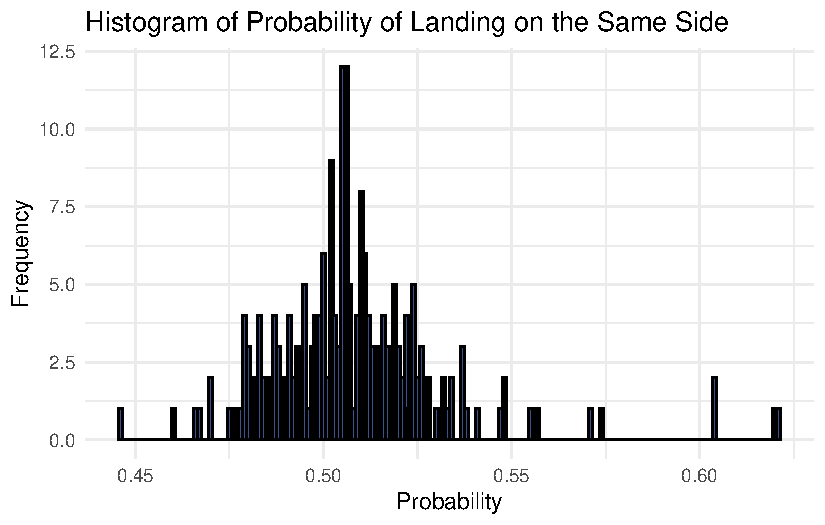
\includegraphics{Garcia-Vuksic-RMProject-2024_files/figure-pdf/unnamed-chunk-4-1.pdf}

\emph{Figure 1: Histogram of the probability of landing on the same side
across all coins and participants.}

Most probabilities cluster around 0.5, but the distribution leans
slightly to the right, reflecting the small bias observed. A few
outliers exceed 0.6, which we will explore further.

\textbf{Participant-Level Analysis}

Next, we examine how this probability varies by participant. Differences
in flipping technique or style could drive variation at the individual
level.

We sum heads-up and tails-up flips by participant to obtain

\$ p\_i =
\frac{(\text{heads_heads})_i + (\text{tails_tails})_i}{(\text{total_flips})_i}\$

where \((\text{heads_heads})_i\) is the total number of heads outcomes
from heads-up starts for participant \(i\), etc.

\begin{verbatim}
# A tibble: 1 x 3
  mean_prob median_prob sd_prob
      <dbl>       <dbl>   <dbl>
1     0.510       0.505  0.0192
\end{verbatim}

The \textbf{mean participant-level probability} is around 0.510,
slightly higher than the overall mean. This minor increase above the
grand mean suggests participants differ in their flipping styles,
possibly through differences in technique or consistency. This is
illustrated in Figure 2.

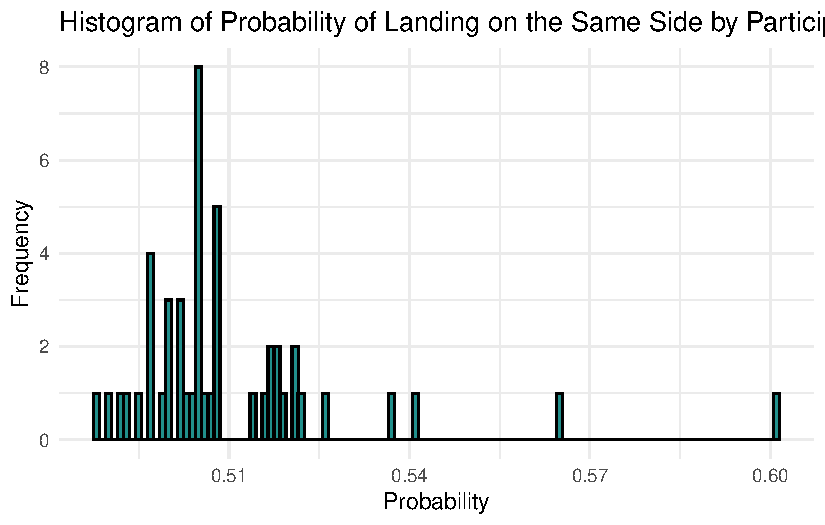
\includegraphics{Garcia-Vuksic-RMProject-2024_files/figure-pdf/unnamed-chunk-6-1.pdf}

\emph{Figure 2: Histogram of Probability of Landing on the Same Side by
Participant}

Although many participants cluster near 0.5, there are some notable
outliers, reinforcing the notion that \textbf{participant-specific
effects} could be important in modeling. We identify outliers by
checking which participants' probabilities lie beyond two standard
deviations from the mean.

\begin{verbatim}
# A tibble: 2 x 8
  person     total_heads_heads total_tails_tails total_heads_up total_tails_up
  <fct>                  <dbl>             <dbl>          <dbl>          <dbl>
1 JanYang                  510               446            877            814
2 TianqiPeng               780               902           1341           1459
# i 3 more variables: total_same_side <dbl>, total_flips <dbl>,
#   prob_same_side <dbl>
\end{verbatim}

\textbf{Coin-Level Analysis}

We then group flips by each \emph{coin} to see whether some coins
inherently land on the same side more frequently. Analogously, we
compute

\(q_j = \frac{(\text{heads_heads})_j + (\text{tails_tails})_j}{(\text{total_flips})_j}\)

where \((\text{heads_heads})_j\) denotes the total number of heads
outcomes from heads-up starts for coin \$j\$, etc.

\begin{verbatim}
# A tibble: 1 x 3
  mean_prob median_prob sd_prob
      <dbl>       <dbl>   <dbl>
1     0.504       0.506  0.0135
\end{verbatim}

The \textbf{mean coin-level probability} is about 0.504, with smaller
overall variability compared to participants, as shown in Figure 3.

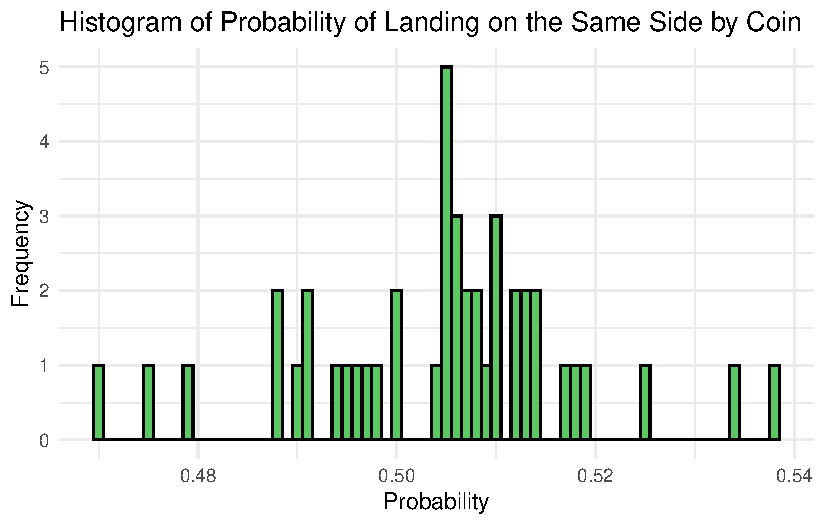
\includegraphics{Garcia-Vuksic-RMProject-2024_files/figure-pdf/unnamed-chunk-9-1.pdf}

\emph{Figure 3: Histogram of the probability of landing on the same side
by coin.}

Coin-level probabilities remain tightly grouped around 0.5. This finding
indicates that, \textbf{on average}, coin characteristics may not
strongly affect the outcome, at least not to the same extent as
participant-specific effects. Outliers were identified for coins with
probabilities exceeding two standard deviations from the mean.

\begin{verbatim}
# A tibble: 4 x 8
  coin    total_heads_heads total_tails_tails total_heads_up total_tails_up
  <fct>               <dbl>             <dbl>          <dbl>          <dbl>
1 0.01GBP               235               240            497            503
2 0.02EUR                78                63            157            143
3 0.50SGD               808               688           1452           1329
4 1MXN                 2215              2292           4177           4257
# i 3 more variables: total_same_side <dbl>, total_flips <dbl>,
#   prob_same_side <dbl>
\end{verbatim}

To further investigate, we analyzed person/coin combinations to explore
whether specific participant-coin interactions exhibit unusual outcomes.

\begin{Shaded}
\begin{Highlighting}[]
\CommentTok{\# Calculate probabilities for person/coin combinations}
\NormalTok{person\_coin\_probs }\OtherTok{\textless{}{-}}\NormalTok{ df }\SpecialCharTok{\%\textgreater{}\%}
  \FunctionTok{group\_by}\NormalTok{(person, coin) }\SpecialCharTok{\%\textgreater{}\%}
  \FunctionTok{summarise}\NormalTok{(}\AttributeTok{prob\_same\_side =} \FunctionTok{mean}\NormalTok{(prob\_same\_side, }\AttributeTok{na.rm =} \ConstantTok{TRUE}\NormalTok{), }\AttributeTok{.groups =} \StringTok{"drop"}\NormalTok{)}

\CommentTok{\# Identify person/coin combination outliers}
\NormalTok{person\_coin\_outliers }\OtherTok{\textless{}{-}}\NormalTok{ person\_coin\_probs }\SpecialCharTok{\%\textgreater{}\%}
  \FunctionTok{filter}\NormalTok{(prob\_same\_side }\SpecialCharTok{\textgreater{}} \FunctionTok{mean}\NormalTok{(prob\_same\_side) }\SpecialCharTok{+} \DecValTok{2} \SpecialCharTok{*} \FunctionTok{sd}\NormalTok{(prob\_same\_side) }\SpecialCharTok{|}
\NormalTok{           prob\_same\_side }\SpecialCharTok{\textless{}} \FunctionTok{mean}\NormalTok{(prob\_same\_side) }\SpecialCharTok{{-}} \DecValTok{2} \SpecialCharTok{*} \FunctionTok{sd}\NormalTok{(prob\_same\_side))}

\FunctionTok{print}\NormalTok{(person\_coin\_outliers)}
\end{Highlighting}
\end{Shaded}

\begin{verbatim}
# A tibble: 9 x 3
  person          coin    prob_same_side
  <fct>           <fct>            <dbl>
1 FranziskaAssion 1EUR             0.557
2 JanYang         0.50EUR          0.604
3 JasonNak        0.50EUR          0.46 
4 MagdaMatetovici 1CAD             0.62 
5 TianqiPeng      0.20EUR          0.621
6 TianqiPeng      0.50EUR          0.604
7 TianqiPeng      1EUR             0.574
8 XiaochangZhao   0.50SGD          0.571
9 XiaoyiLin       0.50EUR          0.446
\end{verbatim}

TianqiPeng and JanYang were identified as outlier participants.

**maybe say something else??? lol im tired and not so sure**

\textbf{Effect of Starting Side}

Finally, we explore whether starting the coin heads-up vs.~tails-up
alters the likelihood of ending on the same side. We compare:

\begin{itemize}
\item
  \(p_{11}=P(Heads→Heads)\)
\item
  \(p_{00}=P(Tails→Tails)\)
\end{itemize}

\begin{verbatim}
# A tibble: 1 x 4
  mean_prob_heads_to_heads mean_prob_tails_to_tails sd_prob_heads_to_heads
                     <dbl>                    <dbl>                  <dbl>
1                    0.508                    0.508                 0.0257
# i 1 more variable: sd_prob_tails_to_tails <dbl>
\end{verbatim}

The results indicate \textbf{both} heads-up and tails-up flips have a
mean probability of about 0.508 of landing on the same side. A t-test
reveals no significant difference between the two groups, implying that
``heads-up'' vs.~``tails-up'' starts do not systematically alter the
bias once participant and coin factors are averaged out.

ive been thinking of how davison said hypothesis tests are overused is
this one of those cases? or is it a reasonable test? i think so but im
also overthinking

\begin{verbatim}
# A tibble: 2 x 3
  starting_side mean_prob sd_prob
  <chr>             <dbl>   <dbl>
1 Heads Up          0.508  0.0257
2 Tails Up          0.508  0.0299
\end{verbatim}

\begin{verbatim}

    Welch Two Sample t-test

data:  probability by starting_side
t = 0.091768, df = 410.93, p-value = 0.9269
alternative hypothesis: true difference in means between group Heads Up and group Tails Up is not equal to 0
95 percent confidence interval:
 -0.005086409  0.005584567
sample estimates:
mean in group Heads Up mean in group Tails Up 
             0.5079109              0.5076618 
\end{verbatim}

A violin plot (Figure 4) shows the distribution of these probabilities:

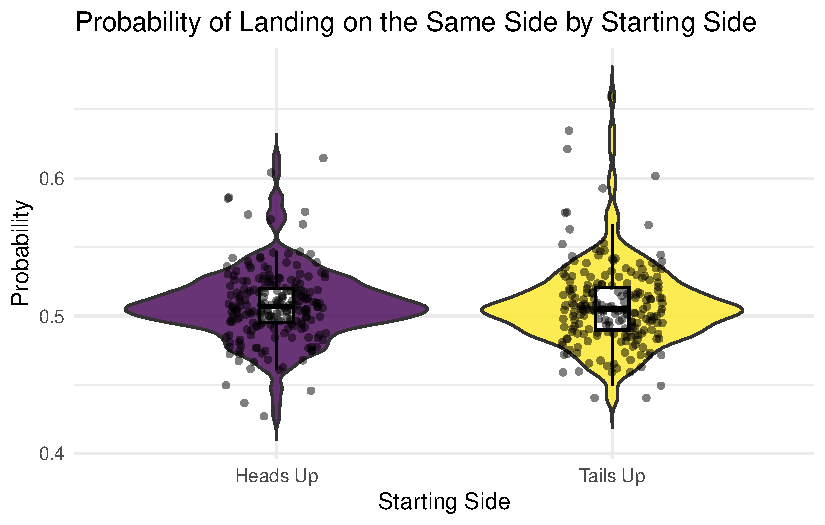
\includegraphics{Garcia-Vuksic-RMProject-2024_files/figure-pdf/unnamed-chunk-14-1.pdf}

\emph{Figure 4: Violin plot of the probability of landing on the same
side by starting side.}

Both distributions are centered around 0.508, with comparable spread,
suggesting \textbf{no notable systematic difference} between starting
heads-up or tails-up. Some outliers in each group do appear, which may
reflect unique participant behaviors or chance fluctuations.

\begin{verbatim}
# A tibble: 21 x 2
# Groups:   starting_side [2]
   starting_side probability
   <chr>               <dbl>
 1 Heads Up            0.446
 2 Heads Up            0.570
 3 Tails Up            0.441
 4 Tails Up            0.602
 5 Tails Up            0.575
 6 Heads Up            0.615
 7 Tails Up            0.593
 8 Heads Up            0.604
 9 Tails Up            0.635
10 Heads Up            0.585
# i 11 more rows
\end{verbatim}

\textbf{Summary of EDA Findings}

\begin{itemize}
\item
  \textbf{Slight Overall Bias}: The mean probability of landing on the
  same side is 0.508, slightly above 0.5, indicating a modest but
  statistically significant bias.
\item
  \textbf{Participant Variability}: A higher mean (0.510) and greater
  spread among participants highlight the importance of
  participant-specific effects. The outliers indicate certain
  participants might be flipping coins in a non-random manner.
\item
  \textbf{Minimal Coin Influence}: Coin-level probabilities are tightly
  clustered around 0.5, suggesting coin characteristics may not play a
  major role ompared to participant influences ---at least in this
  aggregated dataset.
\item
  \textbf{Starting Side}: Heads-up or tails-up leads to virtually the
  same probability (0.508), indicating little difference in bias by
  orientation.
\end{itemize}

These observations will guide the model-building phase. In particular,
\textbf{participant effects} seem important, whereas coin effects appear
weaker. Although starting side does not show a strong effect overall, we
may still retain it in our models to capture any subtle differences.

\hypertarget{analysis}{%
\paragraph{\texorpdfstring{\textbf{3.
Analysis}}{3. Analysis}}\label{analysis}}

Building upon the insights from our EDA, we proceed to model the
probability of a coin landing on the same side using generalized linear
models (GLMs). Given the binary nature of the outcome (landing on the
same side or not), logistic regression is an appropriate choice. We
begin with a simple model and later incorporate hierarchical structures
to account for variability.

\hypertarget{simple-logistic-regression-model}{%
\subparagraph{Simple Logistic Regression
Model}\label{simple-logistic-regression-model}}

As a first step, we fit the simplest possible logistic model, treating
\textbf{all flips} (aggregated in \texttt{df}) as independent Bernoulli
trials with a single intercept term. Conceptually, this model estimates
a single probability \$p\$ that a flip lands heads, irrespective of
participant or coin. Though extremely simplistic, it provides a baseline
for more complex models.

Let \(Y\_{ij}\) denote the number of same-side outcomes for the \(i\)-th
participant-coin pair under starting orientation \(j\), and let
\(m_{ij}\) represent the total flips under these conditions. A simple
logistic regression assumes:
\(\text{logit}\bigl(P(Y_{ij} = 1)\bigr) = \beta_0\) where
\(\beta_0 \in \mathbb{R}\) is the log-odds of landing on the same side,
irrespective of participant, coin, or starting orientation. The
likelihood for \(\beta_0\) is: \$ L(\beta\emph{0) =\prod{i,j}
\binom{m_{ij}}{Y_{ij}} \pi\^{}\{Y}\{ij\}\} (1 - \pi)\^{}\{m\_\{ij\} -
Y\_\{ij\}\}\$ where \(\pi = \frac{\exp(\beta_0)}{1 + \exp(\beta_0)}\).
The maximum likelihood estimate \$\hat{\beta}\emph{0\$ is obtained by
solving \$ \max}\{\beta\emph{0\} \sum}\{i,j\} Y\_\{ij\} \log(\pi) +
(m\_\{ij\} - Y\_\{ij\}) \log(1 - \pi)\$

\begin{verbatim}

Call:
glm(formula = cbind(heads_heads, N_start_heads_up - heads_heads) ~ 
    1, family = binomial, data = df)

Coefficients:
            Estimate Std. Error z value Pr(>|z|)    
(Intercept) 0.031366   0.004783   6.558 5.44e-11 ***
---
Signif. codes:  0 '***' 0.001 '**' 0.01 '*' 0.05 '.' 0.1 ' ' 1

(Dispersion parameter for binomial family taken to be 1)

    Null deviance: 284.28  on 210  degrees of freedom
Residual deviance: 284.28  on 210  degrees of freedom
AIC: 1739.6

Number of Fisher Scoring iterations: 3
\end{verbatim}



\end{document}
